\section{简易Transformer模型的构建过程}\label{sec-5}

本节主要介绍如何构建简易的Transformer模型。需要注意的是,本节的重点在于介绍我们自定义的Transformer及各个模块,因此对于如何调用数据集和训练模型没有做过多的阐释。在下一节中,我们将重点介绍如何利用更复杂更多样的数据集进行模型训练以及如何通过选择不同数据集写出不同风格和类型的诗词。

在本项目中,我们试图只使用Pytorch库中的线性层等简单的模块,自己实现Transformer的相应机制和模块,构建一个能够根据输入的前半句古诗输出后续内容的Transformer。

在实现上,我参考了kaggle上\href{https://www.kaggle.com/code/alionsss/pytorch-transformer-x/notebook}{PyTorch示例——使用Transformer写古诗}的项目架构,挪用了其数据集、编码器、位置编码的实现和整体框架。

\texttt{./code/classes.py }中提供了所有类定义的实现(包含上述数据集和编码器);./trans.ipynb中提供了整个模型的全流程实现。

\subsection{模块类型的定义}

下面我们逐模块的介绍我们的自定义类。

\subsubsection{关于批次的处理}

在第\ref{sec-3}节中,我们并未关注到批次的相关信息。但在实际训练中,通常会使用多批次训练的方法,使得更加有效的利用现有计算资源,提高计算效率和收敛效果。因此我们需要使得构建的模块能够适用于多批次的训练。幸运的是,Pytorch提供了Dataloader处理批次数据,但仍然需要注意在计算损失函数、提供掩码时,需要根据实际情况将张量变形或扩展成相应的具有batch\_size的形状。

在后续内容中,如无特别说明,不再叙述处理批次导致的形状变化。

\subsubsection{嵌入层}

嵌入层主要用于将一个序列转化为编码器、解码器的输入,请关注\texttt{classes.py}中的Embedding类。

具体来讲,对于一个序列长度为$s$,词典大小为$v$的形状为$(s,)$的序列输入,每个位置的值代表一个汉字,我们首先将其转化为形状为$(s,v)$的独热向量,再经过线性层$(v,h)$,得到形状为$(s,h)$的嵌入向量。

\subsubsection{注意力模块}

请关注\texttt{classes.py}中的Attention类。

自注意力和交叉注意力机制的逻辑实质上是相同的,只是在调用时需要使用不同的输入参数。因为本项目中只会使用到自注意力和交叉注意力机制,因此我们假定要么$q,k,v$的输入相同,要么$k,v$的输入相同。

具体实现中,首先我们需要考虑如何实现多头注意力机制。如果我们将数据分别训练$a$次,再将结果拼接在一起,实现复杂度上比较高。

通过探索发现,我们可以将所有$a$个头的$W_Q^i,W_K^i,W_V^i$拼接在一起,使用和单头注意力机制相同的逻辑计算$Q,K,V$,以$Q_i$为例
$$
[Q_1, Q_2,\cdots , Q_a] = [XW_Q^1 , XW_Q^2 , \cdots, XW_Q^a ] = X[W_Q^1, W_Q^2, \cdots, W_Q^a],
$$
这样在代码实现上更加简洁和高效。

之后通过Pytorch提供的view()/permute()/transpose()/expand()等方法,\textbf{将注意力头数作为单独的维度提取出来},再使用矩阵乘法等算子计算即可。

这也体现了在底层实现上基础算子的可扩展性,以矩阵乘法为例,其默认行为是计算输入的后两个维度的矩阵乘积,这使得能够计算更多维的张量的矩阵乘积。

另一点想要额外说明的是,\textbf{注意力机制不要求$q,k,v$\footnote{用小写字母代表原始输入而非经过$W_Q,W_K,W_V$变换后得到的$Q,K,V$。}的维数相等},交叉注意力机制中编码器输出$X:(src_s,h)$和解码器输入$Y:(tgt_s,h)$的维数也可以不相同,仍然可以进行注意力的计算:
\begin{align*}
    Q &=X W_Q , \ &(tgt_s,h) = (tgt_s, h) \times (h,h) \\
    K &=X W_Q , \ &(src_s,h) = (src_s, h) \times (h,h) \\
    V &=X W_Q , \ &(src_s,h) = (src_s, h) \times (h,h) \\
    Z &= \text{softmax}(\frac{QK^T}{\sqrt{h}}) V, \ &(tgt_s, h) = (tgt_s, h) \times (h, src_s) \times (src_s, h),
\end{align*}
此时我们的注意力输出$Z$仍然和需要迭代计算的编码器输入$Y$维度相同,因此能够进行若干层解码器的计算。


\subsubsection{掩码}

请关注\texttt{classes.py}中的Transformer类中关于mask的部分,部分实现如图\ref{fig:simpletT-mask}。

\begin{figure}[h]
    \centering
    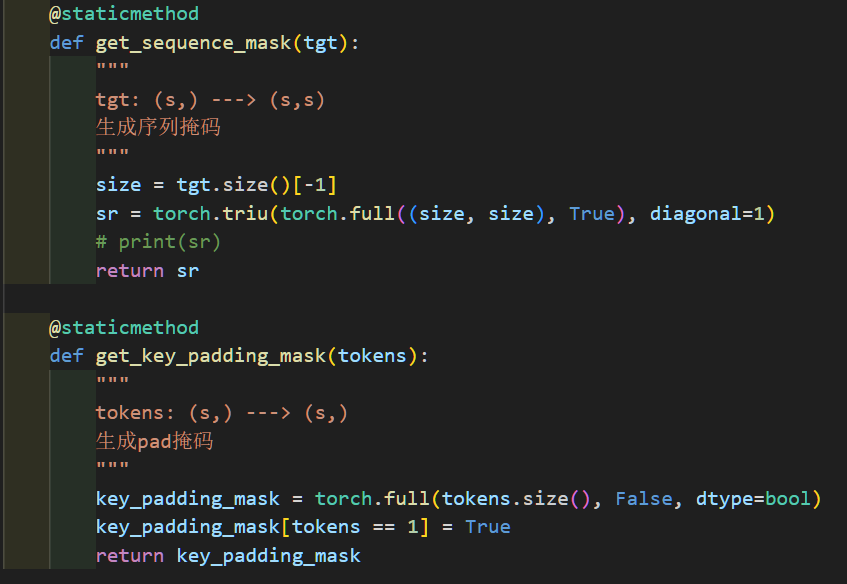
\includegraphics[width=0.8\linewidth]{img/simpleT/simpleT-mask.png}
    \caption{两种掩码的实现}
    \label{fig:simpletT-mask}
\end{figure}

由于我们使用了批量训练,同一批次的数据的序列长度可能不同,但在训练过程中我们将这一个参数进行了固定,因此我们需要调整数据使得同一批次的数据的序列长度相同。

我们采取在数据末尾填充相应的“PAD”符号作为填充占位符来解决这一问题。但这会引发又一个问题,模型可能将“PAD”作为出现频次较高的字符进行学习,进而导致预测输出中大量输出“PAD”。为此,我们需要把模型的注意力从“PAD”上面拿走。这里“拿走”的行为和在遮蔽未来信息的行为是一致的,在实现上,只需在计算softmax之前将这些位置上置$-\infty$,计算出来的结果这些位置上就会是$0$。

此外我们还需要实现在\label{sec-2:mask}中提到的针对解码器自注意力输入的掩码。另外,在实现过程中我还思考了交叉注意力为什么不需要遮蔽未来信息:在交叉注意力中,查询(Query)来自解码器的当前状态,而键(Key)和值(Value)来自编码器的输出。编码器的输出是已经处理好的特征向量,这些特征向量之间没有时间顺序的依赖关系,而查询Q相互之间是“独立的”,因此交叉注意力不需要防止未来信息的泄露。

\subsubsection{TransformerEncoderDecoder模块}

请关注\texttt{classes.py}中的TransformerEncoderDecoder类。

在这里,我们实现了Transformer模型的主要模块,提供自定义编码器、解码器的层数,注意力的头数,掩码,前馈神经网络隐层维度等。

在这里需要关注的是,交叉注意力机制中,解码器的输入(也就是交叉注意力机制的$k,v$)来自于解码器输出的最后一层,而非每个解码器层的输出。这进一步表明,解码器和编码器在Transformer架构中是两个相对独立的结构。

\subsubsection{其他}

\paragraph{残差连接}

这里的实现和原理比较简单,残差连接的具体实现在TransformerEncoderDecoder类中,这里我们实现了改进策略中Layernorm的结构调整(\ref{sec-4:ln-adjust}),可以在调用时指定norm\_first参数来决定使用哪一种Layernorm,如果\texttt{norm\_first == True},则使用Pre-LN Transformer layer。

\paragraph{层归一化} 请关注\texttt{classes.py}中的LayerNorm类。在此我们只关注一个点,在实现层归一化时,不应假定矩阵的维数,而是直接将其最后一层归一化即可,这样提高了我们代码的可复用性和可扩展性。

\paragraph{全连接前馈神经网络} 请关注\texttt{classes.py}中的FeedForward类。这里我们提供了两种可选的激活函数,部分实现了\ref{sec-4:nonlinear-activation}中的改进策略,分别是RELU和GELU。
\\

除了以上类外,还有一些较为简单的类,比如位置编码(PositionalEncoding类)、预测层(Prediction类)等,不再赘述。

\paragraph{模型构建} 请关注\texttt{classes.py}中的Transformer类,我们将所有需要的模块分别初始化后,通过前向传播路径拼装到一起,构成最终的Transformer模型。我们还在这个类中为注意力模块添加了默认掩码。

\subsection{模型训练和表现}

将上述模块集成为Transformer后,我们使用./data/poetry.txt中的诗词数据,$\texttt{batch\_size} = 64$, 编码器和解码器层数为$3$,注意力头数$a=4$,迭代$\texttt{epoch} = 50$轮,采取交叉熵损失,进行训练和预测。每轮的损失函数如图\ref{fig:simpleT-loss},预测效果如图\ref{fig:simpleT-performance}。
\begin{figure}[h]
    \centering
    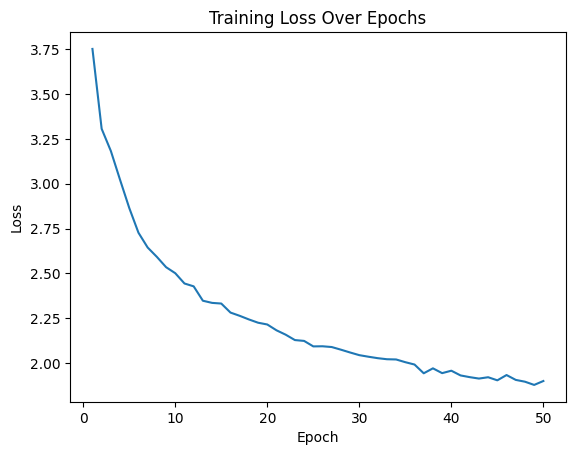
\includegraphics[width = 0.55\textwidth]{img/simpleT/simpleT-loss.png}
    \caption{损失函数变化}
    \label{fig:simpleT-loss}
\end{figure}

\begin{figure}[h]
    \centering
    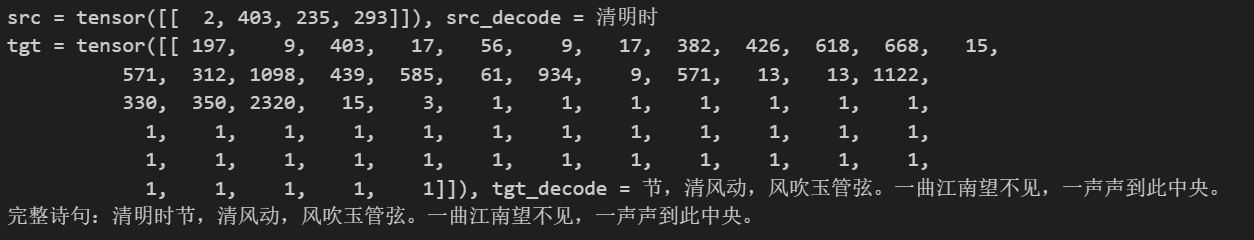
\includegraphics[width = \textwidth]{img/simpleT/simpleT-performance.png}
    \caption{模型预测表现}
    \label{fig:simpleT-performance}
\end{figure}

如希望进行类似测试,可以在\texttt{./trans.ipynb}中运行“模型训练”上方所有单元格(类定义和超参数)及“存储模型”(绘制损失函数之后)下方所有单元格(加载模型参数和预测),即可在避免训练的情况下进行相应测试。

\subsection{构建过程中的问题和解决}

在构建模块中,遇到了若干问题,虽然Transformer的架构和注意力机制的计算在原理上已经比较熟悉,但实现过程中仍然出现了许多意料不到的场景,这里简要介绍一下。

\subsubsection{如何执行单元测试}

对于简单的函数和类,我们可以通过构造测试样例等检验函数是否实现了相应功能,但对于嵌套和调用结构复杂的类来讲,如何去验证其行为是否相符,困扰了我相当长的一段时间。

在刚写完相应模块的代码时,我的思路是比较我实现的类和Pytorch提供的类在训练过程中的收敛速度,从而判断实现是否正常,不过这种方法虽然能够发现收敛速度有较大差异,但无法定位到具体的模块,实际上仍需要手动检查每个块的内部逻辑。

经过较长时间的试错后,我发现可以\textbf{针对每个模块,提供相同的输入给我的实现和Pytorch的实现,并且在模型初始化后,指定模型的参数相同,避免参数初始化的随机性影响结果,再比较他们的输出是否相同,以此来判断模块是否正常。}在机器学习中,如果像数学证明中验证两个对象是否相等的逻辑,的确很难进行,但这种排除随机性,验证相同输入下输出是否相同的方法反而是有效和易用的。

\texttt{./code/Comparision.ipynb} 实现了上述自定义模块和Pytorch相应模块的检验。

\subsubsection{维度验证}

在课程学习矩阵求导相关知识时,对于矩阵求导是否正确,课程Note中使用维度进行检验,这依然不符合我的直觉,认为这只能提供一个非常基本和低层次的检验。但在这次作业中,我深刻意识到了维度检验这一方法的重要性和实用性。

Pytorch提供的接口能够便捷的改变张量的形状,但与二维矩阵不同的时,考虑到批次和注意力头数的参与,张量的形状往往可能是三维甚至四维的,在这种情况下,简要运算过程中不同变量的维度信息,能够很方便的检验整个运算过程是否符合我们的预期。

我们以注意力模块为例,展示在实现过程中的维度验证(图\ref{fig:simpleT-dimension})。
\begin{figure}[h]
    \centering
    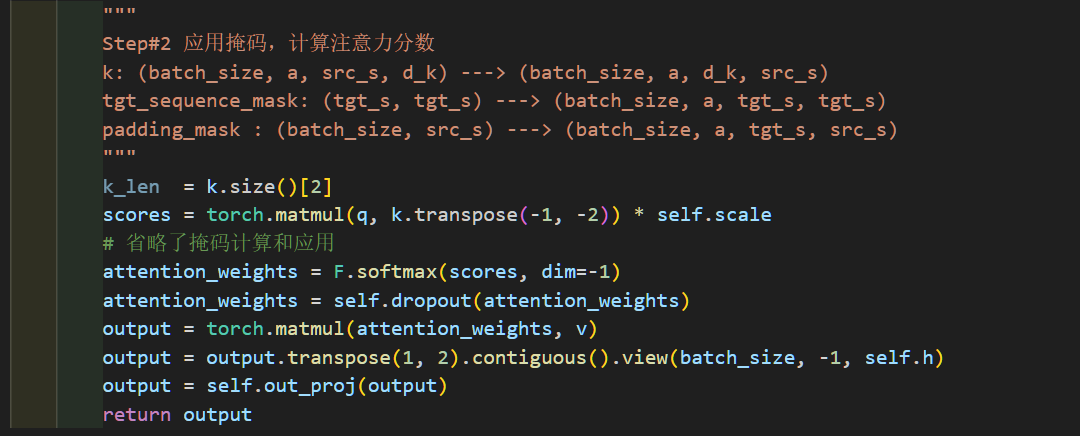
\includegraphics[width=\linewidth]{img/simpleT/simpleT-dimension.png}
    \caption{维度验证在注意力计算中的应用}
    \label{fig:simpleT-dimension}
\end{figure}

\subsubsection{模块的可复用性}

通过类这种面向对象的编程方式,我们能够复用我们定义好的模块。不过python无法导入定义在\texttt{.ipynb}文件中的方法,因此,我们将所有的类定义单独封装在.\texttt{/classes.py}中,可以通过在其他文件中\texttt{from classes import *}复用我们的类和方法,也方便了后续进行的古诗文写作助手的进一步优化和封装。

另一方面,通过定义多个子模块,我们可以像积木一样任意的拼接各个模块,从而产生不同结构的模型,进行不同的尝试,这也是面向对象编程的一大乐趣。

\subsubsection{如何开发新功能}

如果在现有代码上直接更改,很有可能出现代码无法正常运行,又无法回退的局面。在这次作业中,我尝试带领小组成员一起使用代码版本管理工具,在一定程度上非常有助于开发新功能、扩展新模块,当出现异常时,能够非常简单的回退到原始状态,或进行对比以发现问题所在。不过比较遗憾的是,小组成员并没有太多git使用经验,当模型初步编写完成后和其他两位同学同步开发时,由于需要更新部分接口或操作逻辑,代码版本的不统一造成了一定困难。

这也提示我们,在编写代码时,需要充分考虑到接口的可扩展性,同时理清模型依赖关系,尽可能清晰的完成新功能开发的每一步。